\documentclass[aps,superscriptaddress,twocolumn,nopreprintnumbers,floatfix,groupedaddress]{revtex4-1}
\usepackage{amssymb}
\usepackage{amsmath}
\usepackage{graphicx}
\usepackage{dcolumn}
\usepackage{hyperref} % tab this to get rid of colored hyper ref
\usepackage{color,units}
\usepackage{lineno}
\usepackage{xspace}
\usepackage{mathtools}
\usepackage{physics}
\usepackage{acronym}
\usepackage{subfigure}
\usepackage{multirow}
\usepackage{tikz}


\newcommand{\bilby}{{\sc Bilby}\xspace}
\newcommand{\lal}{{\sc LAL}\xspace}
\newcommand{\lalsuite}{{\sc LALSuite}\xspace}
\newcommand{\lalsimulation}{{\sc LALSimulation}\xspace}
\newcommand{\sur}{{\sc NRHybSur3dq8}\xspace}
\newcommand{\Z}{\mathcal{Z}}
\newcommand{\M}{\mathcal{M}}
\renewcommand{\L}{\mathcal{L}}
\newcommand{\BF}{\mathcal{BF}}
\newcommand{\proposal}{proposal}
\newcommand{\target}{target}
\newcommand{\ep}[1]{\textcolor{red}{[EP: #1]}}
\newcommand{\et}[1]{\textcolor{blue}{[ET: #1]}}
\newcommand{\ct}[1]{\textcolor{green}{[CT: #1]}}


\newcommand{\emcee}{{\sc emcee}\xspace}
\newcommand{\ptemcee}{{\sc ptemcee}\xspace}
\newcommand{\nessai}{{\sc Nessai}\xspace}
\newcommand{\vitamin}{{\sc VItamin}\xspace}
\newcommand{\bilbypipe}{{\sc bilby\_pipe}\xspace}
\newcommand{\lalinference}{{\sc LALInference}\xspace}
\newcommand{\dynesty}{{\sc dynesty}\xspace}
\newcommand{\cpnest}{{\sc cpnest}\xspace}
\newcommand{\nflows}{{\sc nflows}\xspace}
\newcommand{\pytorch}{{\sc PyTorch}\xspace}
\newcommand{\corner}{{\sc corner}\xspace}
\newcommand{\matplotlib}{{\sc matplotlib}\xspace}
\newcommand{\seaborn}{{\sc seaborn}\xspace}
\newcommand{\numpy}{{\sc NumPy}\xspace}
\newcommand{\scipy}{{\sc SciPy}\xspace}
\newcommand{\pandas}{{\sc pandas}\xspace}
\newcommand{\python}{{\sc Python}\xspace}
\newcommand{\imrphenomp}{{\sc IMRPhenomPv2}\xspace}
\newcommand{\pycbc}{{\sc PyCBC}\xspace}


\newcommand{\figwidth}{8.6cm}
\newcommand{\onehalffigwidth}{12.9cm}
\newcommand{\doublefigwidth}{17.2cm}
\newcommand{\montefigwidth}{11cm}
\newcommand*{\checktikz}[1][]{\tikz[x=1em, y=1em]\fill[#1] (0,.35) -- (.25,0) -- (1,.7) -- (.25,.15) -- cycle;}
\raggedbottom
\setlength{\parskip}{0pt}

\begin{document}

\raggedbottom

\title{Explainable Deep-learning: Monte Carlo methods for Gravitational-Wave Inference}

\author{Project No:~628}
\affiliation{%
	SUPA, School of Physics and Astronomy \\
	University of Glasgow \\
	Glasgow G12 8QQ, United Kingdom}%

\date{\today}

\begin{abstract}
A wonderful serenity has taken possession of my entire soul, like these sweet mornings of spring which I enjoy with my whole heart. I am alone, and feel the charm of existence in this spot, which was created for the bliss of souls like mine. I am so happy, my dear friend, so absorbed in the exquisite sense of mere tranquil existence, that I neglect my talents. I should be incapable of drawing a single stroke at the present moment; and yet I feel that I never was a greater artist than now. When, while the lovely valley teems with vapour around me, and the meridian sun strikes the upper surface of the impenetrable foliage of my trees, and but a few stray gleams steal into the inner sanctuary, I throw myself down among the tall grass by the trickling stream; and, as I lie close to the earth, a thousand unknown plants are noticed by me: when I hear the buzz of the little world among the stalks, and grow familiar with the countless indescribable forms of the insects and flies, then I feel the presence of the Almighty, who formed us in his own image, and the breath of that universal love which bears and sustains us, as it floats around us in an eternity of bliss; and then, my friend, when darkness overspreads my eyes, and heaven and earth seem to dwell in my soul and absorb its power, like the form of a
\end{abstract}

\maketitle

\acrodef{GW}[GW]{Gravitational wave}
\acrodef{BBH}[BBH]{binary black hole}
\acrodef{EM}[EM]{electromagnetic}
\acrodef{CBC}[CBC]{compact binary coalescence}
\acrodef{BNS}[BNS]{binary neutron star}
\acrodef{NSBH}[NSBH]{neutron star black hole}
\acrodef{PSD}[PSD]{power spectral density}
\acrodef{ELBO}[ELBO]{evidence lower bound}
\acrodef{LIGO}[LIGO]{advanced Laser Interferometer Gravitational wave Observatory}
\acrodef{CVAE}[CVAE]{conditional variational autoencoder}
\acrodef{KL}[KL]{Kullback--Leibler}
\acrodef{GPU}[GPU]{graphics processing unit}
\acrodef{LVC}[LVC]{LIGO-Virgo Collaboration}
\acrodef{PP}[p-p]{probability-probability}
\acrodef{SNR}[SNR]{signal-to-noise ratio}

\section{Introduction}\label{intro}

From their first hypothesis~\cite{einstein1} to the first direct detection of signal from binary black hole coalescence~\cite{abbott2016observation} by Advanced LIGO~\cite{advancedLIGO} and Advanced VIRGO~\cite{advancedVIRGO} square-kilometre interferometers, we find ourselves in an exciting new epoch of gravitational physics. (change this last phrase).

As theorised in general relaitivty gravitational waves are stretching and deformation of space-time from rotating massive objects. Sources can be spilt into two types: continuous grav waves (CWs) and transient grav wave signals (GWs). There is Much ongoing work concerning Cws \cite{bayley2019soap} and even significant effort to implement deep-learning techniques \cite{bayley2020soapML,cwml2019} however this paper solely focuses on GW transients, in particualr from compact binary coalesnecs (CBCs)

CBCs are stellar mass objects either black holes or lighter NS rotate and coalsence in 3 stages known as inspiral,ringdown and merger (IMR) as they merge the distotions of spacetime occur at such a frequency that they can be detected by a network of ground-based detector, where the distrotions leave a precious impriment on detector strain of laser interferomters called a waveform. 

Intro detector network, 2nd gen, getting ready for (Future additions to network – Japan KAGRA~\cite{kagra}, INDIA~\cite{UNNIKRISHNAN_2013} etc. (need citations)), introduce the idea of waveform banks (links to the specific template banks of next subseciton), observing run of transients (need to stress the main observations are CBCs), sensitive frequency band. Observe through a process of matched filtering using specific detection pipelines PyCBC~\cite{pycbc2016} and GstLal (gen1 - \cite{gstlal_gen1_2017}, gen2 - \cite{gstlal_gen2_2019}), by comparing incoming observed detector strain pattern to a bank of modelled templated waveforms, modelled by solving GR equations using computational modelling technique numerical relativity. 

Having completed both o3 runs the detectors are currently undergoing improvements in prep for o4 run with more detectors added (mention more detectors being added) and increased detector sensitivity there is much more CBCs going to be detected and Observing runs are just for Gwtransients. With the first two observing runs~\cite{BBHo1,gwtc1} and the first half of the third run~\cite{gwtc2} findings published along with corresponding public data release, the field of GW research find itself at the forefront of new science. 

\subsection{Parameter Estimation}

Intro PE + params, (link to first 2 cols of Table 1) (already introduced waveform in prev section, can build straight from that) 

PE relies on bayesian inf with relaies on Bayesian Stats...(3eqns) – introduce usefulness of bayesian evidence.

Bayesian inference in practise – software is BILBY, LALinference, PyCBCInference \cite{lalinference,PyCBCInference,bilby} algorithms are MCMC or NS – Ns is more verstaile as it can evalute Bayesian Evidence also (already explained why that’s useful) samplers are…. Dont need to list the samplers here, just the refs and link to table 2.

Motivation for fast and accurate PE at the end – MM astronomy(gw170817) (birth of MMA, detectors sensitive enough to detect NS – only going to get more and more)(Motivates fast PE), Hubble constant etc. (Motivates accurate.) and subsection2 – really need to re invent the PE method as detector sensitivty gets better – to push new sceince leading edge.

Whilst these methods are accurate, they struggle with speed, table 2 shows on order 10 hours to generate a meaningful sample batch from posterior. (even with some clever software to speed up by order of 2 (2 hunter refs under his speed table) its too slow)

This speed element does motivate deep-learning approaches to speed up sampling rate post training. Much work has been done deep-learning for all steps of GW DA \cite{mlreview2020}, in paritclaur PE with some software opting to enhance current sampling methods \cite{williams2021nested}, we present a method to completely replace old tehcniques, using a tehcnique called VI \cite{1904.06264} which circumvents costly likelihood cals to produce a meaningful batch of samples in subsecond run-times post-training.



%
\begin{table}[t]
	\centering
	\caption{The full parameter range of CBC PE presented alongside the subset of inferred parameters highlighted with prior boundary values.}
	\begin{tabular}[t]{lcccc}
		\toprule
		parameter name & symbol & status & value & units\\
		\hline
		mass 1 & $m_1$ & inferred  & 35-80 & \(\textup{M}_\odot\)\\
		mass 2 & $m_2$ & inferred & 35-80 & \(\textup{M}_\odot\)\\
		luminosity distance & $d_{\text{L}}$ & inferred & 1-3 & Gpc\\
		time of coalescence & $t_{0}$ & inferred & 0.65-0.85 & s\\
		inclination & $\Theta_{jn}$ & inferred & 0-$\pi$ & rad\\
		polarisation & $\psi$ & inferred & 0-$\pi$ & rad\\
		\hline
		right ascension & $\alpha$ & fixed & 0 & rad\\
		declination & $\delta$ & fixed & 0 & rad\\
		spins & - & fixed & 0 & -\\
		\hline
		phase at coalescence & $\phi_{0}$ & marginalised & 0-$2\pi$ & rad\\
		\botrule
	\end{tabular}
	\label{tab:params}
\end{table}
%
%
%
\begin{align}\label{eq:bayes_exact} 
	p(x|y) = \frac{{\cal L}(y|x) p(x)}{\cal Z} ,
\end{align}

\begin{align}\label{eq:bayes_evidence} 
{\cal Z} = \int dx {\cal L}(y|x) p(x) ,
\end{align}

\begin{align}\label{eq:bayes_prop} 
	p(x|y) &\propto {\cal L}(y|x) p(x). 
\end{align}


%
%Need to know if equation is at end of sentence then swap comma for full stop
%
%
%
\subsection{Deep-learning Approaches}

Intro DL as a whole/premise/computational technique – introduce the term hyperparams.

A specific type of DL NN is generative model which have been shown to be good for approximate inference from incomplete data \cite{1807.03653,bond2021deep} a recent comparative analysis of gen models <--

Much work has been done on gen models with two in particular being well suited for our task

Norm flows – descibe breifly uses Nns to learn an invertiblelinear mapping from original distribution to unit normal which is easier to sample from – 

VAEs – breifly describe – uses encoder and decoder networks to map input distribution to lower dim latent space dim and reconstructs from there.

Norm flows has been shown to be very successful in this task \cite{williams2021nested,stephengreen2020,papamakarios2019normalizing} However, due to faster training and similar sample quality (from bond2021 – word nicely) we opted to use a VAE for our VI task, aptly names Vitamin.

%
\subsection{\vitamin: User-friendly Inference}\label{vit}
%
\begin{align}\label{eq:cross_ent} 
H(p,r) &= -\int dx\, p(x|y) \log r_{\theta}(x|y),
\end{align}

\begin{align}\label{eq:prop_post}
r_{\theta}(x|y) = \int dz\,r_{\theta_1}(z|y)r_{\theta_2}(x|y,z).
\end{align}

We present vit, state follow on work from hutner’s paper and name is paper 1
Start with more specific intro of what CVAE is with figure straight away (caption following from hutner’s paper)

2 equations, talk about right hand side of fig1 only (training is in methods), put the proposal posterior equation first!something like – to train the model we look to minimise the cost function: (eq) which is minimised when our porposal posterior tends to our true posterior.(footnote – notation both true and target posteriors use p(x|y) the true posterior is used in training/validation only whereas the targter posterior in this paper comes from old school dynesty sampler) Will talk more about training in Section~\ref{methods:model training}.

(remember punctuation after equations)

Compare speed to others (table 2 – normflows with VI stephen green) from table 2 we can see the large jump in run timeusing VI compared to other techniques. 

However using VI limits versatility for speed, so we present a method to estimate likeloods of proposal posterior samples using Monte Carlo methods.

Having the ability to evaluate likelihoods open the door for many useful applications such as evaluating the Bayesian evidence as in equation 3. A particularly useful application called likelihood was shown to be successful in~\cite{OzGrav}. In this paper they used an approximate waveform generator~\cite{IMRPhenomD} to generate a proposal posterior using the Bilby implementation of cpnest and reweigh it according to likelihood ratios with a more complete, but computationally expensive, waveform generator~\cite{NRHybSur3dq8} using a process called sampling-importance resampling (SIR)~\cite{brian2006resampling}. They found by rewighting the likelihoods of the two distierbutions, they could effectively simulate sampling from the target posterior without having to ever run sampler on computationally expensive waveforms.

Once we have estimated our proposal likelihoods, we look to e use a similar SIR approach to reweigh our samples according to their likleihood ratio relative to our target posterior evaluated using the Bilby implementation of dynesty to improve the results of vitamin.

The structure of the paper is as follows. 


Signposting:

In Section 2 we discuss the methods behind training our model in our reduced parameters space and desicbe monte carlo methods for likleihood evaluation and reweighting. In Section 3, we discus the quality of these proposal likelihoods using qualitative sle-consistency and quantitative reproducibility tests. We then go on to evaluate the suitability of the SIR method for our resampling compared to the success of \cite{OzGrav}. Finally, in Section 4, we contextualise our results in the wider field of rapid PE by DL and reiterate the significance of added versatility of vitamin and set out the roadmap of related future work.

\begin{table}[t]
	\centering
	\caption{Required run-times for traditional and DL sampling methods to produce benchmark posterior estimate.}
	\begin{tabular}[t]{l|lcc} 
				\toprule
				sampler & algorithm & deep-learning & run-time (s)\footnote{The benchmark for posterior estimate is $\mathcal{O}(10000)$ samples. Run-times for DL algorithms do not include training time.}\\
				\hline
				\emcee~\cite{emcee} & MCMC~\cite{mcmc_og} & X  &  32070\\
				\ptemcee~\cite{ptemcee} & MCMC & X & 24372\\
				\hline
				\dynesty~\cite{dynesty} & NS~\cite{skilling2006} & X & 19400\\
				\cpnest~\cite{cpnest} & NS & X &  26202 \\
				\nessai~\cite{williams2021nested} & NS & \checktikz & 9372\\
				\hline
				flows~\cite{stephengreen2020} & VI~\cite{1904.06264} & \checktikz & 2\\
				\vitamin~\cite{vitpaper} & VI & \checktikz & $1\times 10^{-1}$\\
				\botrule
	\end{tabular}
	\label{tab:speed}
\end{table}

%
%
%Use gen pap to intro CVAE in context, CONTEXT IS KEY HERE
%
%
\begin{figure}
	\centering
	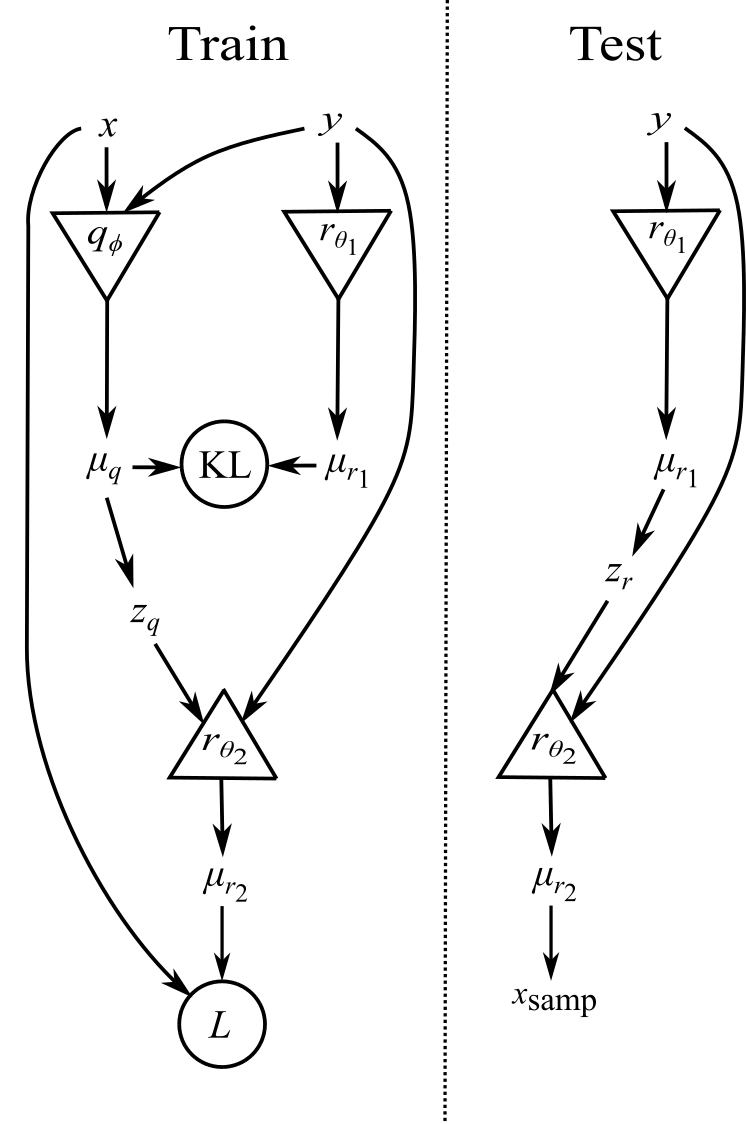
\includegraphics[width=\figwidth]{figs/network_setup.png}
	\caption{The structure of the \ac{CVAE}
		neural network. During training (left-hand side), a training set of noisy
		\ac{GW} signals ($y$) and their corresponding true parameters ($x$) are given
		as input to encoder network $q_{\phi}$, while only $y$ is given to
		encoder network $r_{\theta_1}$. The output of the decoder ($\mu_x$) describes a distribution in
		the physical parameter space and the cost component $L$ is computed by
		evaluating that distribution at the location of the original input $x$.
		When performed in batches this scheme allows the computation of the total cost
		function Eq.~\ref{eq:cost_approx}. After having trained the network and
		therefore having minimised the cross-entropy $H$, we test (right-hand side)
		using only the $r_{\theta_1}$ encoder and the $r_{\theta_2}$
		decoder to produce samples ($x_{\text{samp}}$). These samples are drawn
		from the proposal distribution $r_{\theta}(x|y)$ (Eq.~\ref{eq:prop_post})
		and accurately model the true posterior $p(x|y)$. Figure sourced from paper 1~\cite{vitpaper}.}
	\label{fig:vit_flow}
\end{figure}

%%
%%\subsection{Structure}
%%
%%\subsection{Training}
%%
%%\subsection{Results}
%
%%\section{Theoretical Framework}\label{theory}
%
%Need to mention metropolis hastings it seems!
%
%Introduce equations directly to our specifics, we don't have space to intro them blind then again to specifics...
%
%%\subsection{Monte Carlo Framework}\label{theory:monte}
%
%%\subsection{SIR Framework}\label{theory:sir}
%
%Do theory on normal IS and then say that SIR is an monte carlo approach/approx to normal IS then give equations for bot (talk about the NEW IMPROVED SIR method (link to Section \ref{future}))
%
%%
%%\subsection{Theoretical Framework}\label{monte:theory}
%
%\section{Methodology}\label{methods}
%
%Apply the intro/theory mateiral to our case, JUSTIFY scientific decisions like number of samples, batch size, npars!!
%
\subsection{Model Training}
%
\begin{align}\label{eq:cost_approx} H \lesssim
\frac{1}{N}\sum_{n=1}^{N_{\text{b}}}&\Big[\overbrace{-\log
	r_{\theta_{2}}(x_{n}|z_{n},y_{n})}^{L}\nonumber\\
&+\overbrace{\text{KL}\left[q_{\phi}(z|x_{n},y_{n})||r_{\theta_{1}}(z|y_{n})\right]}^{\text{KL}}\Big],
\end{align}
%
%
\begin{figure}
	\centering
	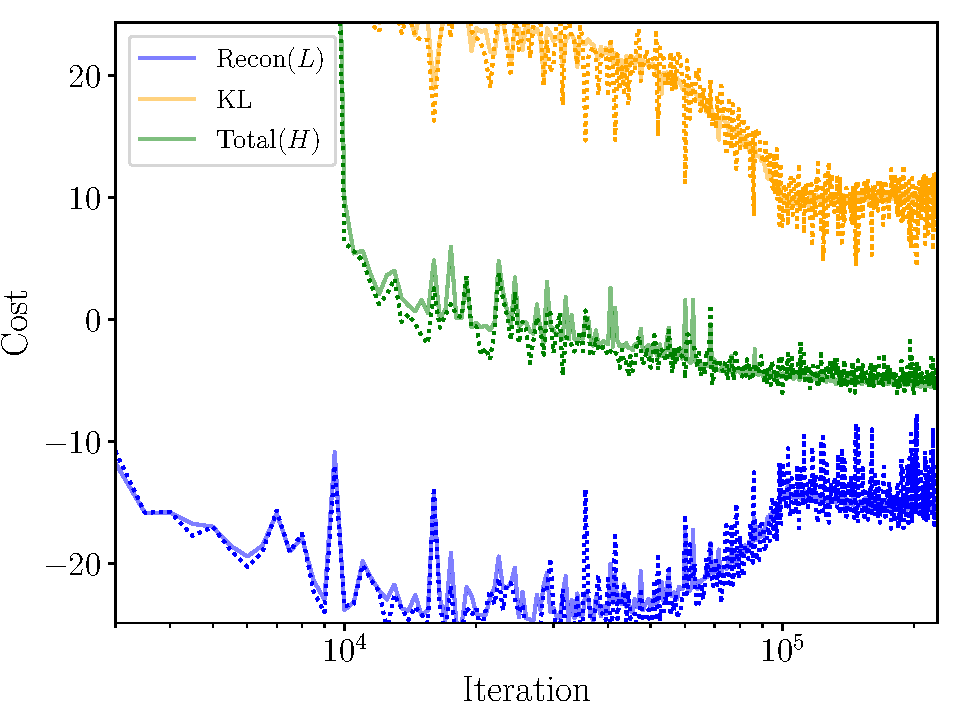
\includegraphics[width=\figwidth]{figs/cost.pdf}
	\caption{}
	\label{fig:learning_contours}
\end{figure}

\begin{figure*}
	\subfigure{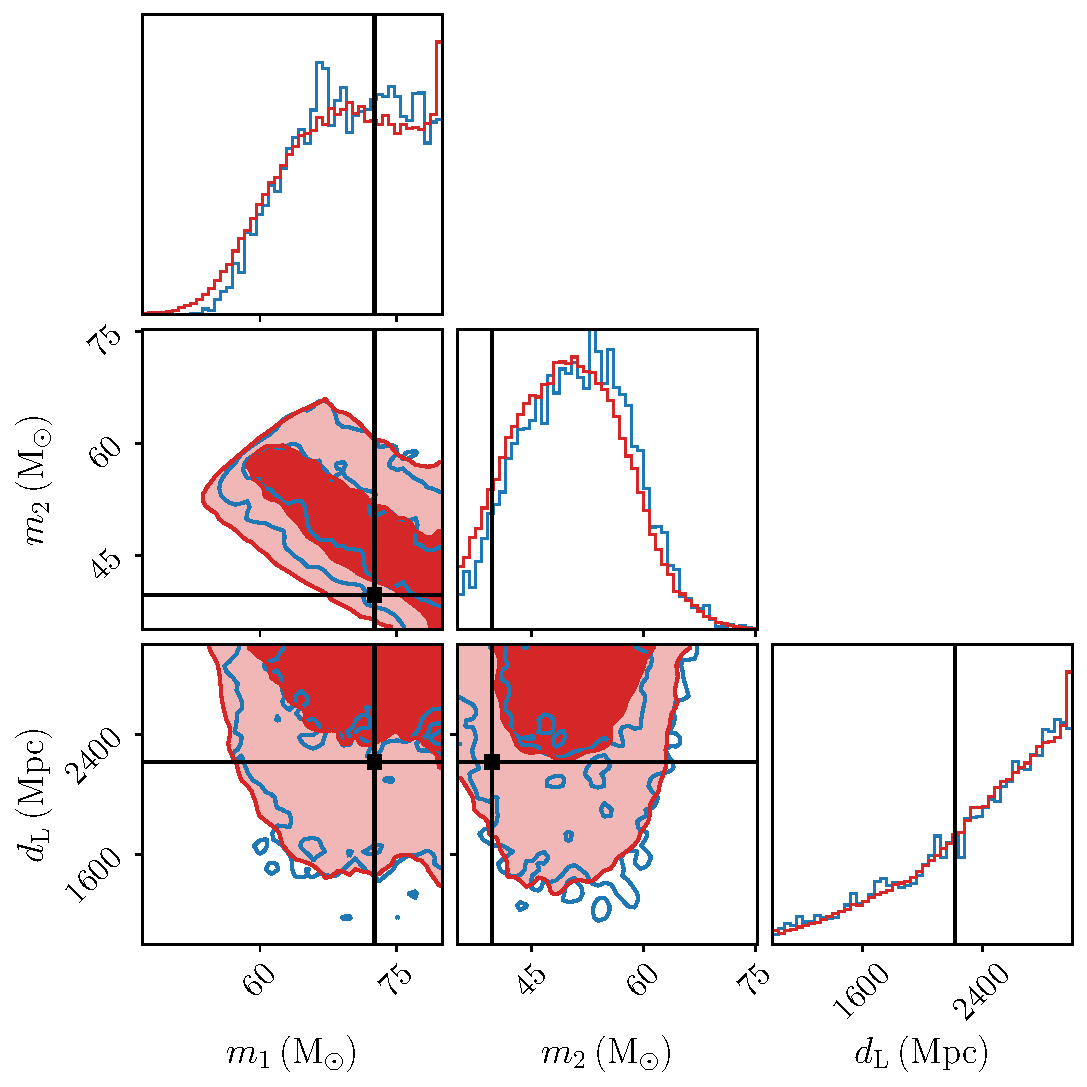
\includegraphics[width=\figwidth]{figs/vit_train_corner1.pdf}}
	\subfigure{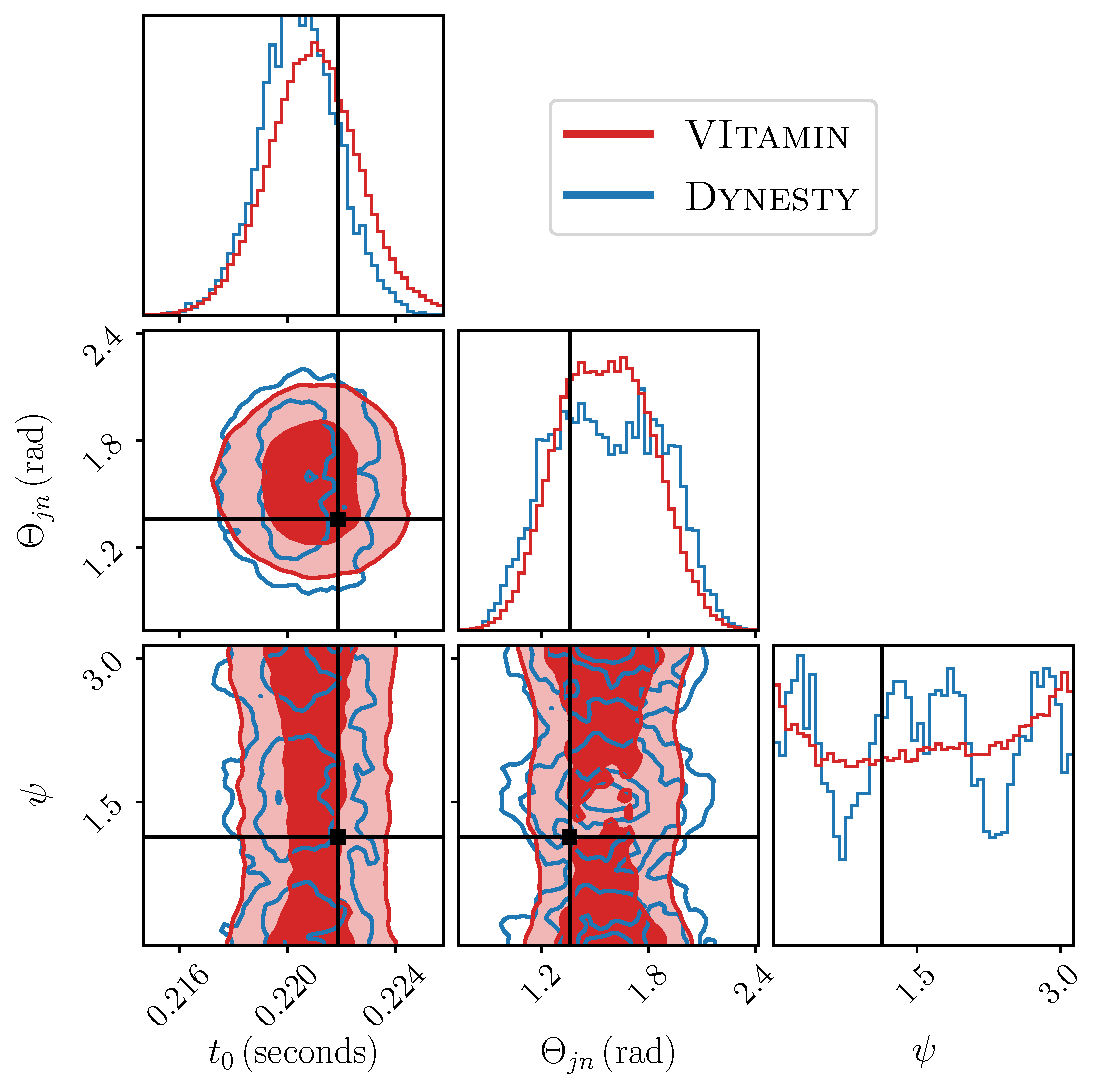
\includegraphics[width=\figwidth]{figs/vit_train_corner2.pdf}}
	\caption{Probability-probability (P-P) plot showing the confidence interval versus the fraction of the events within that confidence interval for the posterior distributions obtained using our analysis \nessai for 128 simulated compact binary coalescence signals produced with \bilby and \bilbypipe. The 1-, 2- and 3-$\sigma$ confidence intervals are indicated by the shaded regions and $p$-values are shown for each of the parameters and the combined $p$-value is also shown.}
	\label{fig:vit_train_corner}
\end{figure*}


\subsection{Likelihood Estimates}

\begin{align}\label{eq:monte_approx}
	r_{\theta}(x|y) = & \,\mathbb{E}_{r_{\theta_1}(z|y)}r_{\theta_2}(x|y,z)\nonumber \\
	 \approx & \frac{1}{N}\sum^{N}_{j=1}\left.r_{\theta_{2,j}}(x_i|y,z_j)\right|_{z_j\sim r_{\theta_1}(z_j|y)},
\end{align}

\begin{align}\label{eq:post_like}
r_{\theta}(x|y) \sim {\cal L}_{\theta}(y|x),
\end{align}

\textbf{\textcolor{red}{Figs: Monte flowchart}}

\begin{figure*}
	\centering
	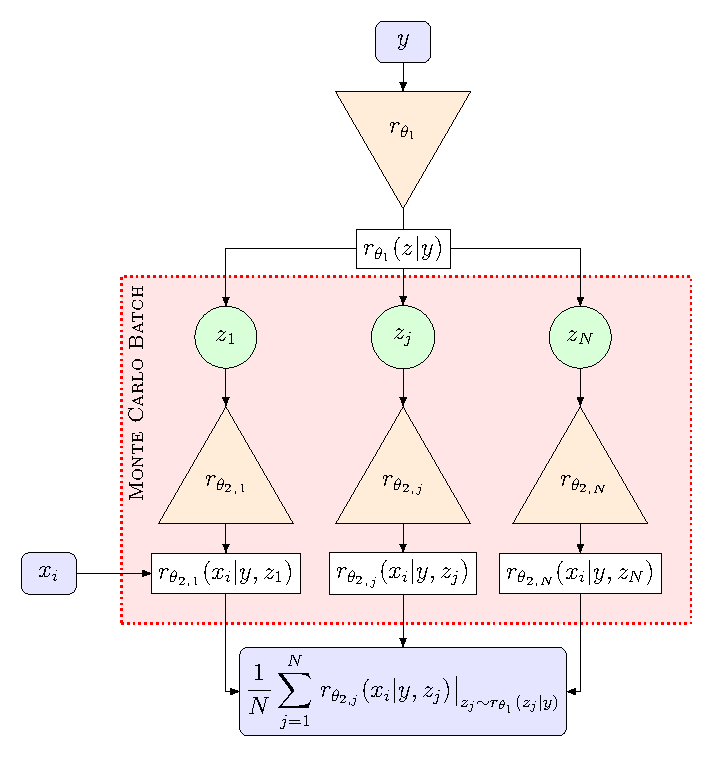
\includegraphics[width=\montefigwidth]{figs/tikz_monte.pdf}
	\caption{}
	\label{fig:monte_flow}
\end{figure*}


\subsection{Likelihood Reweighting}

Start with eq 2 then multiply by unity

\begin{align}\label{eq:sir} 
p(x|y) &\propto \frac{{\cal L}_\theta(y|x)}{{\cal L}_\theta(y|x)}{\cal L}(y|x) p(x)\nonumber\\
&\propto w(y|x)\overbrace{{\cal L}_{\theta}(y|x) p(x)}^{r_{\theta}(x|y)}.
\end{align}

%\begin{table}
%	\centering
%	\caption{Med time to gen 10,000 samples...the DL doesnt account for training time}
%	\begin{tabular}[t]{llcc} 
%				\toprule
%				sampler & method & deep-learning & run-time (s)\\
%				\hline
%				h &&&\\
%				h &&&\\
%%				\emcee~\cite{mcmc_og} & help & help & help\\
%%				help & & &\\
%%				\emcee~\cite{mcmc_og} & help & help & help\\
%%				\emcee~\cite{emcee} & MCMC~\cite{mcmc_og} & X  &  32070\\
%%				\ptemcee~\cite{ptemcee} & MCMC & X & 24372\\
%%				\dynesty~\cite{dynesty} & NS~\cite{skilling2006} & X & 19400\\
%%				\cpnest~\cite{cpnest} & NS & X &  26202 \\
%%				\hline
%%				\nessai~\cite{williams2021nested} & NS & Y & 9372\\
%%				\vitamin~\cite{vitpaper} & VI~\cite{1904.06264} & Y & $1\times 10^{-1}$\\
%				\botrule
%	\end{tabular}
%	\label{Tab:speed}
%\end{table}
Here,

\begin{align}\label{eq:weights}
w(y|x) \equiv \frac{{\cal L}(y|x)}{{\cal L}_{\theta}(y|x)},
\end{align}

is the weight function...

\section{Results}\label{results}

\subsection{Self-consistency}

\begin{figure*}
	\subfigure{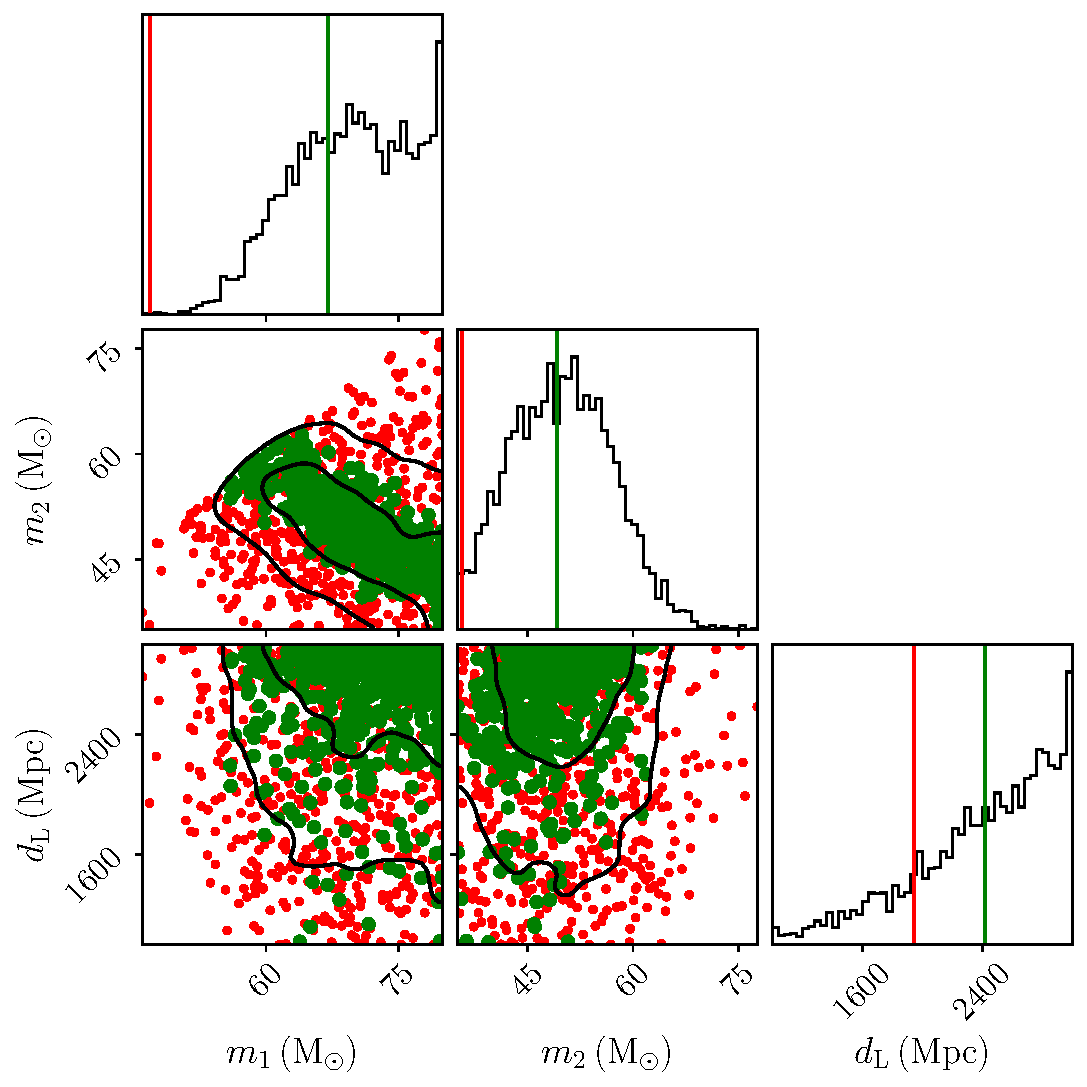
\includegraphics[width=\figwidth]{figs/self_consist1.pdf}}
	\subfigure{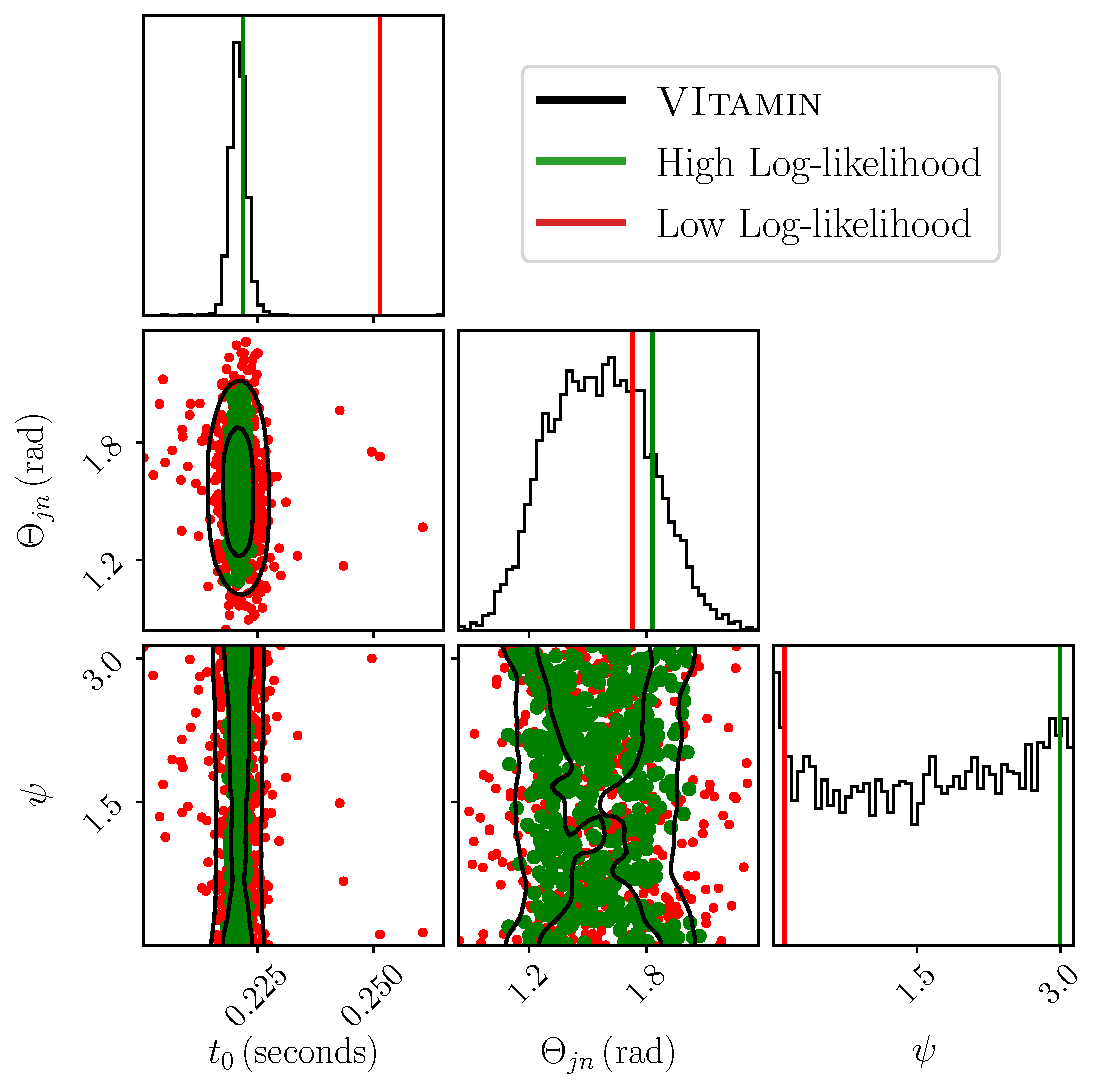
\includegraphics[width=\figwidth]{figs/self_consist2.pdf}}
	\caption{Probability-probability (P-P) plot showing the confidence interval versus the fraction of the events within that confidence interval for the posterior distributions obtained using our analysis \nessai for 128 simulated compact binary coalescence signals produced with \bilby and \bilbypipe. The 1-, 2- and 3-$\sigma$ confidence intervals are indicated by the shaded regions and $p$-values are shown for each of the parameters and the combined $p$-value is also shown.}
	\label{fig:sel_consist}
\end{figure*}


\subsection{Reproducibility}

\begin{align}\label{eq:sigma}
\sigma \propto \frac{1}{\sqrt{N}},
\end{align}

where N is monte carlo batch size

\begin{align}\label{eq:error}
\text{Error} = \frac{\sigma}{\sqrt{n_{\text{samples}}}},
\end{align}



\begin{figure}
	\centering
	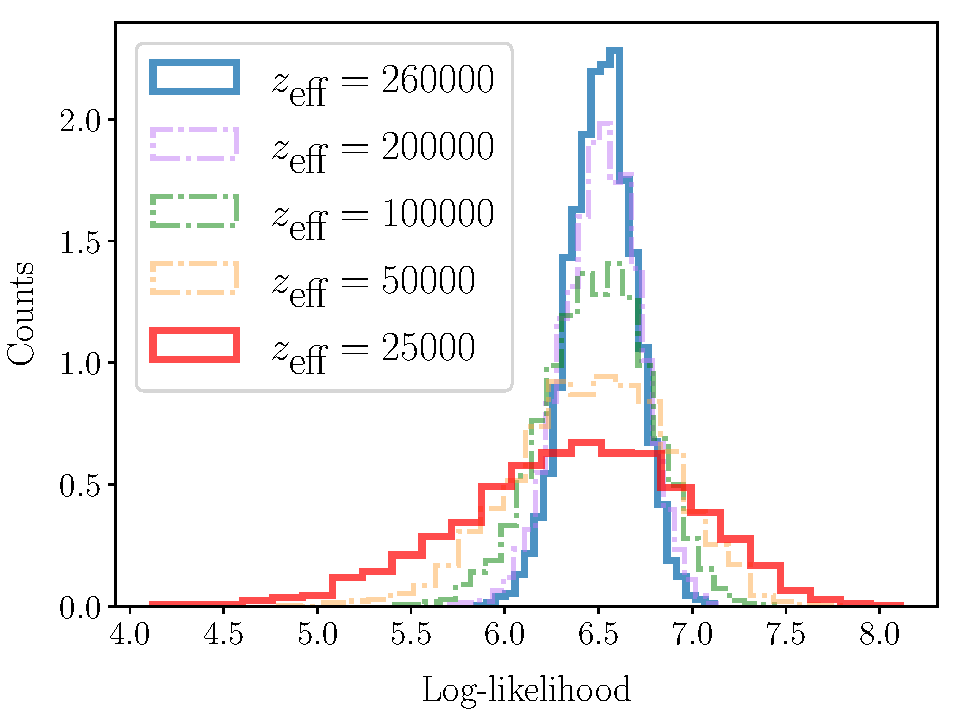
\includegraphics[width=\figwidth]{figs/hists_rect.pdf}
	\caption{}
	\label{fig:hists}
\end{figure}

\begin{figure*}
	\subfigure[]{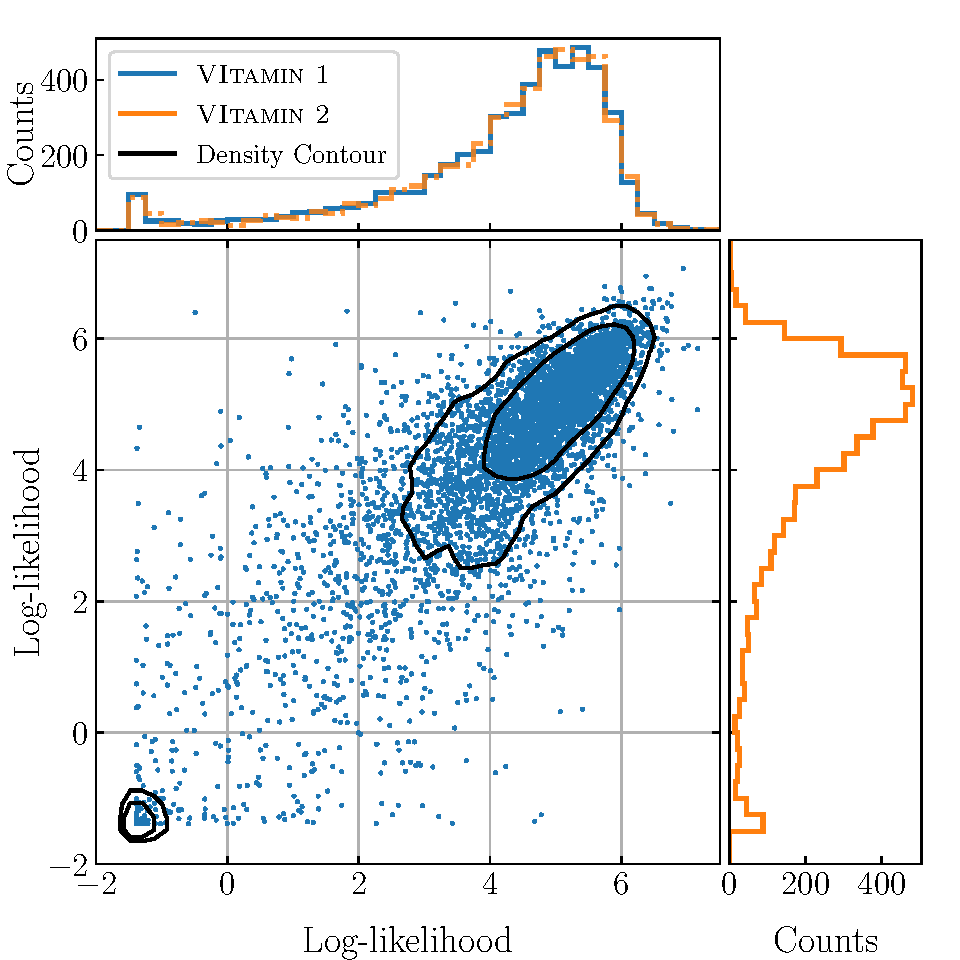
\includegraphics[width=\figwidth]{figs/vvscatter.pdf}}
	\subfigure[]{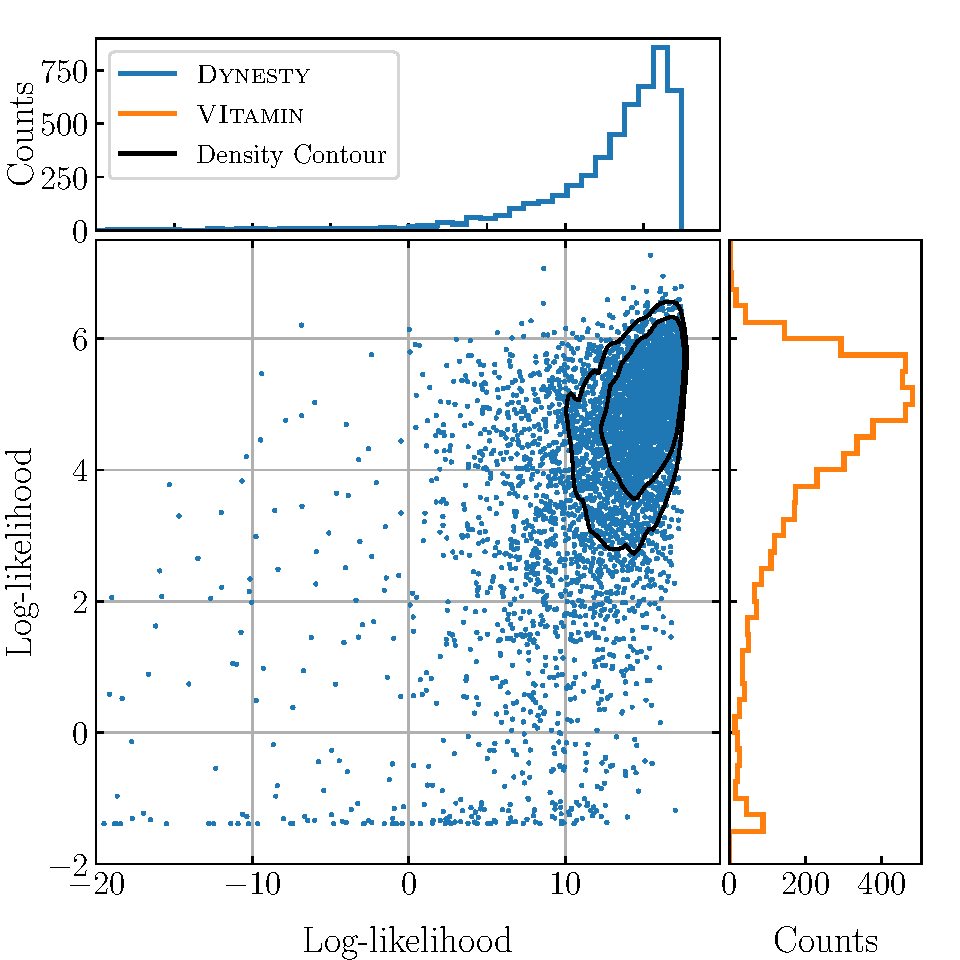
\includegraphics[width=\figwidth]{figs/bvscatter.pdf}}
	\caption{Probability-probability (P-P) plot showing the confidence interval versus the fraction of the events within that confidence interval for the posterior distributions obtained using our analysis \nessai for 128 simulated compact binary coalescence signals produced with \bilby and \bilbypipe. The 1-, 2- and 3-$\sigma$ confidence intervals are indicated by the shaded regions and $p$-values are shown for each of the parameters and the combined $p$-value is also shown.}
	\label{fig:scatter}
\end{figure*}

\subsection{Importance Resampling}


\begin{figure*}[h]
	\centering
	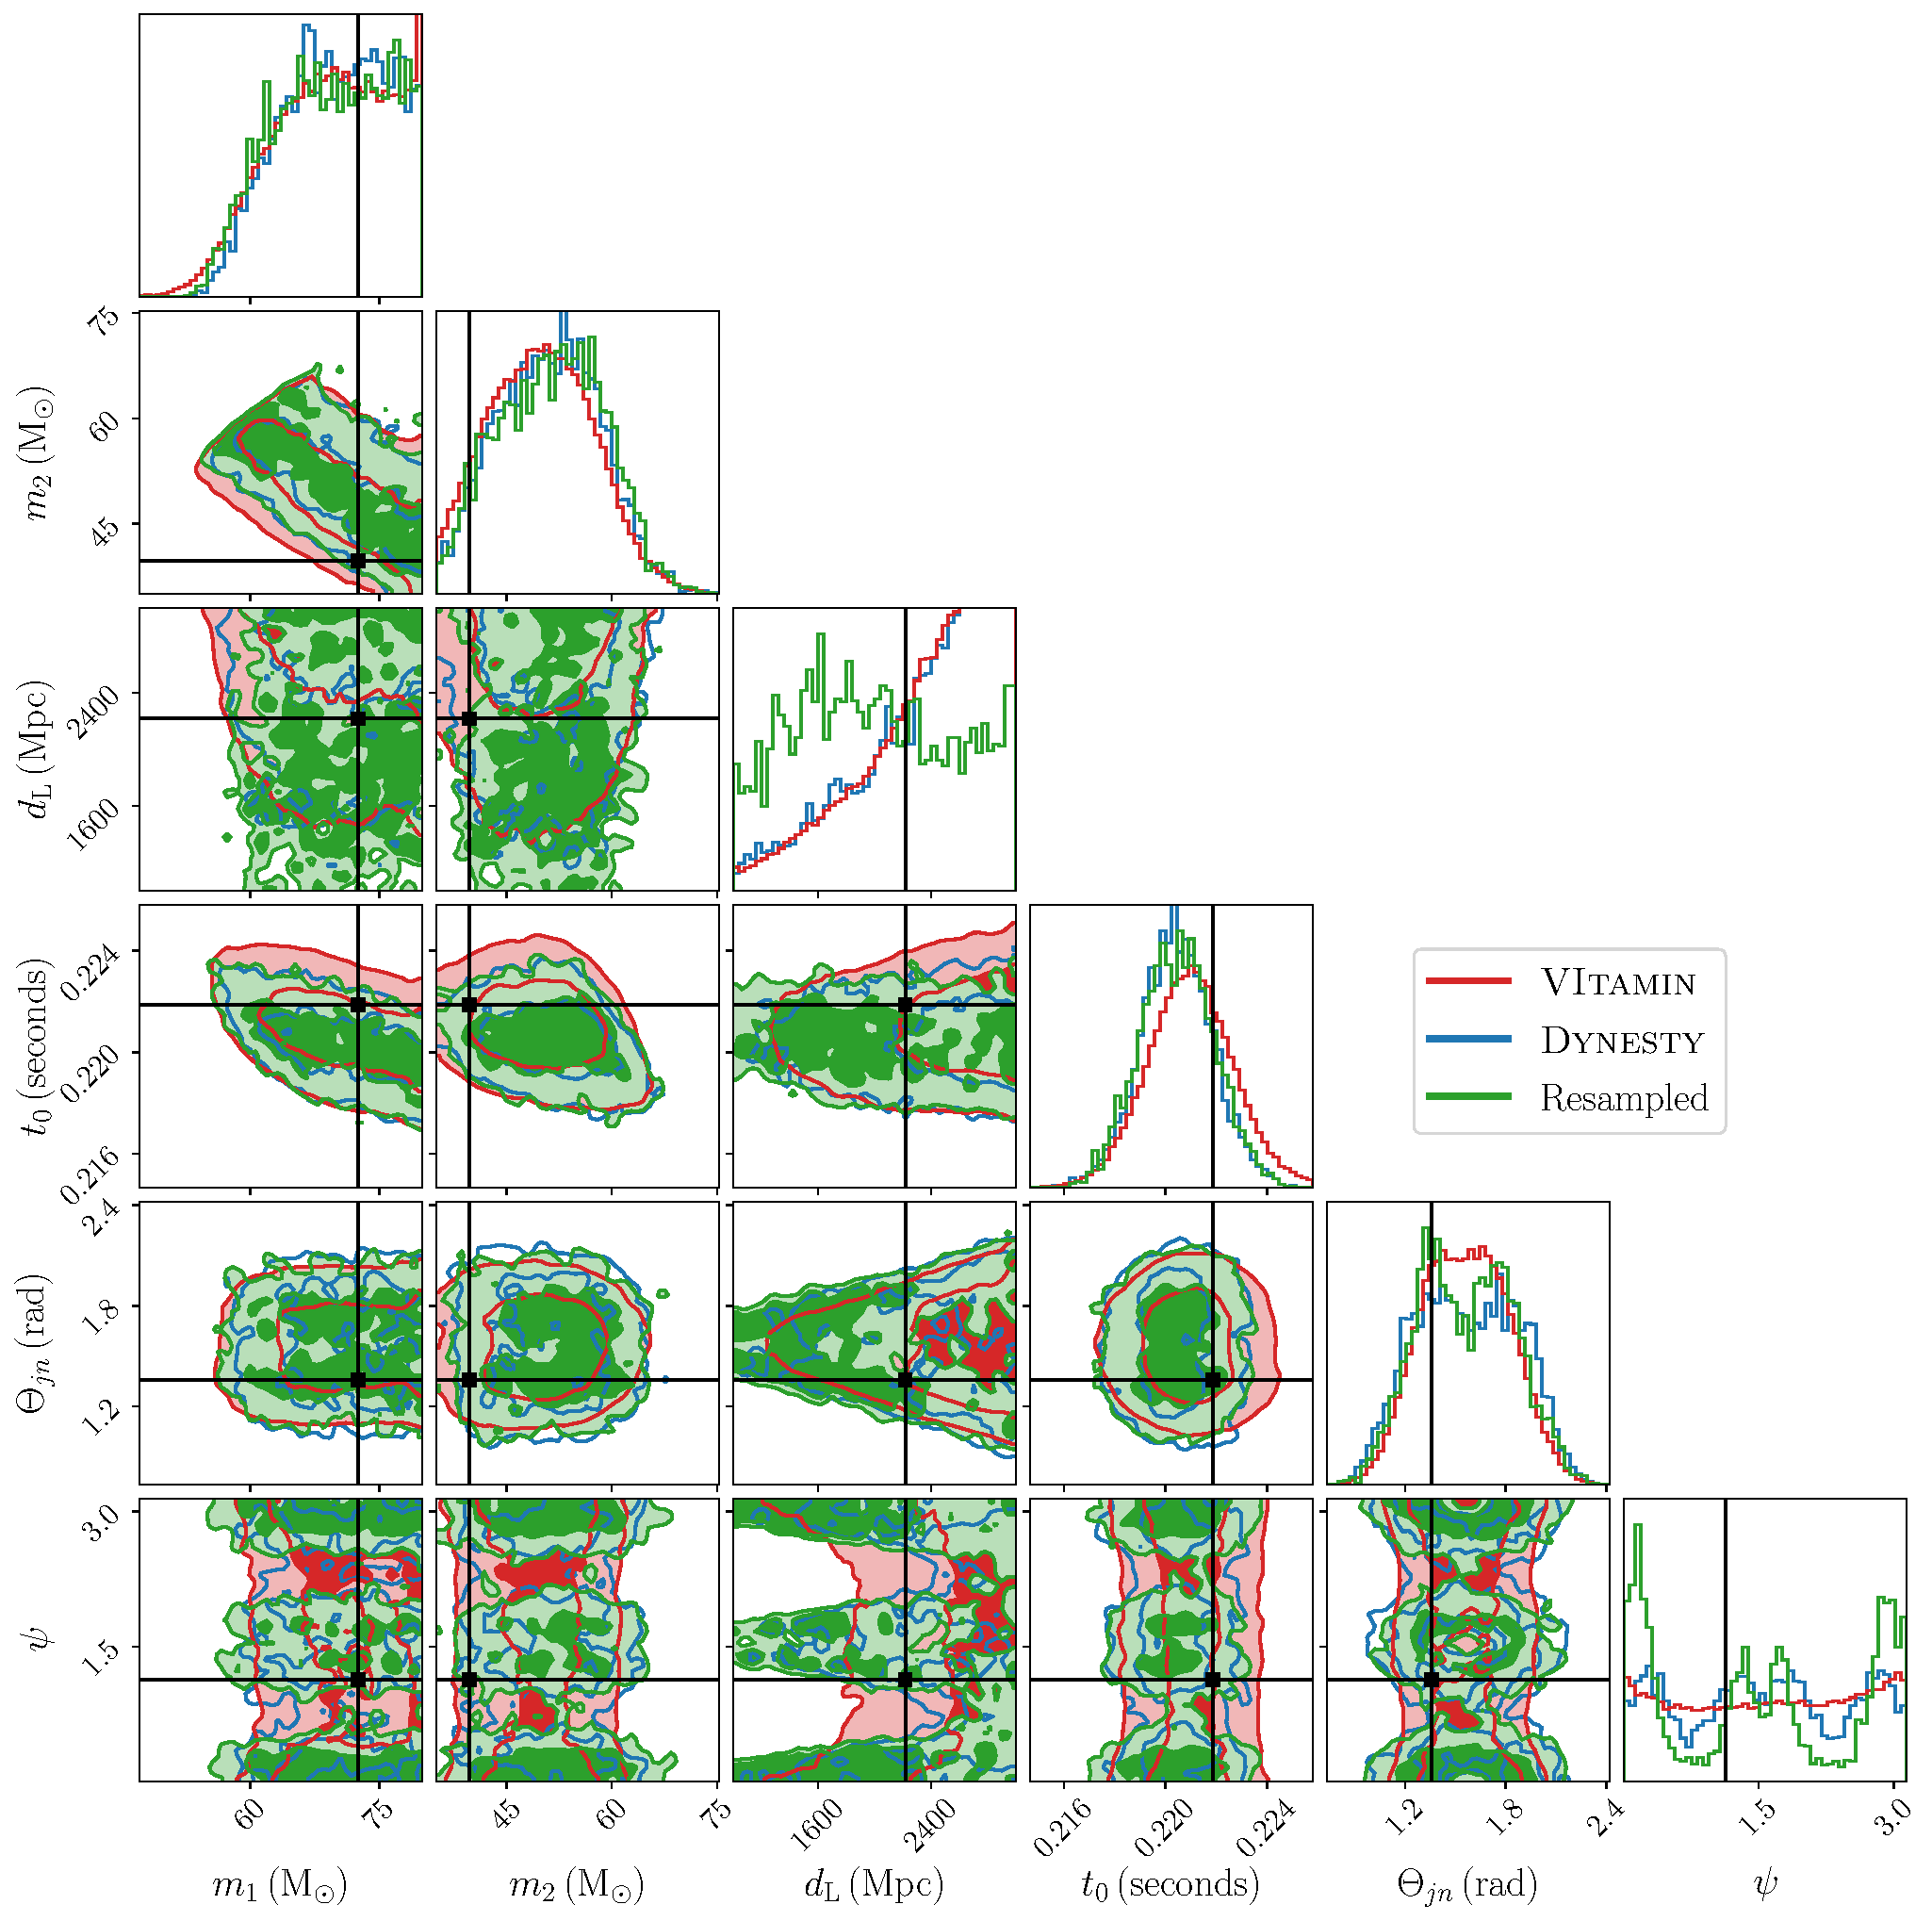
\includegraphics[width=\doublefigwidth]{figs/resample_corner.pdf}
	\caption{}
	\label{fig:final_corner}
\end{figure*}

%\section{Future Work}\label{future}


\section{Conclusions}\label{conc}

This is section has to encapsulate everything we did so that after the abstract a reader can go here and see if they want to buy the paper or not!

As we find ourself in a proof-of-concept mode, there is justification of a section dedicated to the next steps leading towards production of this code.


\section*{Acknowledgements}

Thanks to Chris and Hunter and Michael and Daniel.

Paragraph on the software used \bilby\cite{bilby} \cite{0004-637X-748-2-136}help please dont fuck up now , lets just keep typing and see what happens, im really shitting ymself now... and dont want to have to spend precious time on fucking type setting and bibliography hunting \cite{emcee}
%%\clearpage
%

%
\cleardoublepage
\bibliography{refs}




\end{document}